%% 
%% Copyright 2007-2024 Elsevier Ltd
%% 
%% This file is part of the 'Elsarticle Bundle'.
%% ---------------------------------------------
%% 
%% It may be distributed under the conditions of the LaTeX Project Public
%% License, either version 1.3 of this license or (at your option) any
%% later version. The latest version of this license is in
%%  http://www.latex-project.org/lppl.txt
%% and version 1.3 or later is part of all distributions of LaTeX
%% version 1999/12/01 or later.
%% 
%% The list of all files belonging to the 'Elsarticle Bundle' is
%% given in the file `manifest.txt'.
%% 
%% Template article for Elsevier's document class `elsarticle'
%% with numbered style bibliographic references
%% SP 2008/03/01
%% $Id: elsarticle-template-num.tex 249 2024-04-06 10:51:24Z rishi $
%%
\documentclass[preprint,12pt]{elsarticle}

%% Use the option review to obtain double line spacing
%% \documentclass[authoryear,preprint,review,12pt]{elsarticle}

%% Use the options 1p,twocolumn; 3p; 3p,twocolumn; 5p; or 5p,twocolumn
%% for a journal layout:
%% \documentclass[final,1p,times]{elsarticle}
%% \documentclass[final,1p,times,twocolumn]{elsarticle}
%% \documentclass[final,3p,times]{elsarticle}
%% \documentclass[final,3p,times,twocolumn]{elsarticle}
%% \documentclass[final,5p,times]{elsarticle}
%% \documentclass[final,5p,times,twocolumn]{elsarticle}

%% For including figures, graphicx.sty has been loaded in
%% elsarticle.cls. If you prefer to use the old commands
%% please give \usepackage{epsfig}

%% The amssymb package provides various useful mathematical symbols
\usepackage{amssymb}
%% The amsmath package provides various useful equation environments.
\usepackage{amsmath}
%% The amsthm package provides extended theorem environments
%% \usepackage{amsthm}
\usepackage{float}
%% The lineno packages adds line numbers. Start line numbering with
%% \begin{linenumbers}, end it with \end{linenumbers}. Or switch it on
%% for the whole article with \linenumbers.
%% \usepackage{lineno}

%% Added by author
% Allow long URLs in references to break at hyphens and other safe points.
\PassOptionsToPackage{hyphens}{url}
\usepackage{hyperref}
\hypersetup{
  pdftitle={Informational Content Analysis of Lost Languages},
  pdfauthor={Richard H. Witt, Anamaria Berea},
  colorlinks=true,   % true: colored links instead of boxes
  hypertexnames=false, % avoid duplicate page anchor names in frontmatter
  linkcolor=blue,   % color of internal links
  urlcolor=blue,    % color of external links/URLs
  citecolor=blue,   % color of citation links
  filecolor=blue,   % color of file links
  pdfborderstyle={/S/U/W 1} % underline links instead of boxes
}
\usepackage[table]{xcolor}    
\usepackage{booktabs}
\usepackage{colortbl}   
\definecolor{A6GreyBlue}{HTML}{5686AA}
\definecolor{A6GreyGrey}{HTML}{7d93a0}
\definecolor{A6LightGrey}{HTML}{E5E9EC}

\journal{TBD}

\begin{document}

\begin{frontmatter}

%% Title, authors and addresses

%% use the tnoteref command within \title for footnotes;
%% use the tnotetext command for theassociated footnote;
%% use the fnref command within \author or \affiliation for footnotes;
%% use the fntext command for theassociated footnote;
%% use the corref command within \author for corresponding author footnotes;
%% use the cortext command for theassociated footnote;
%% use the ead command for the email address,
%% and the form \ead[url] for the home page:
%% \title{Title\tnoteref{label1}}
%% \tnotetext[label1]{}
%% \author{Name\corref{cor1}\fnref{label2}}
%% \ead{email address}
%% \ead[url]{home page}
%% \fntext[label2]{}
%% \cortext[cor1]{}
%% \affiliation{organization={},
%%       addressline={},
%%       city={},
%%       postcode={},
%%       state={},
%%       country={}}
%% \fntext[label3]{}

\title{Informational Content Analysis of Lost Languages}

%% Alternative title 1: if I add budget analysis
%%\title{Science, Policy, and Money: How Science gets funded in the United States}

%% use optional labels to link authors explicitly to addresses:
%% \author[label1,label2]{}
%% \affiliation[label1]{organization={},
%%       addressline={},
%%       city={},
%%       postcode={},
%%       state={},
%%       country={}}
%%
%% \affiliation[label2]{organization={},
%%       addressline={},
%%       city={},
%%       postcode={},
%%       state={},
%%       country={}}

\author[1]{Richard Witt\corref{cor1}}
\ead{rwitt4@gmu.edu}

\author[2]{Anamaria Berea}
% \ead{aberea@gmu.edu}

\affiliation[1]{organization={Computational and Data Sciences, PhD Student,George Mason University},
      addressline={4400 University Drive}, 
      city={Fairfax},
      postcode={22030}, 
      state={Virginia},
      country={USA}}

\affiliation[2]{organization={Computational Social Sciences, Associate Professor, George Mason University},
      addressline={4400 University Drive}, 
      city={Fairfax},
      postcode={22030}, 
      state={Virginia},
      country={USA}}

\cortext[cor1]{Corresponding author}

%%%%%%%%%%%%%%%%%%%%%%%%%%%%%%%%%%%%%%%%%%%%%%%%%%%%%%%%%%%%%%%%%%%%%%%%%%%%%%%%%%%
% Abstract
%%%%%%%%%%%%%%%%%%%%%%%%%%%%%%%%%%%%%%%%%%%%%%%%%%%%%%%%%%%%%%%%%%%%%%%%%%%%%%%%%%%
\begin{abstract}
%% Text of abstract

This study investigates what information can be recovered from symbolic data such as lost languages. It compares two exploratory approaches that require no prior knowledge of the data. Machine learning clustering and information theoretic measurements. HDBSCAN is used to uncover recurring groups without predefined categories.  Information theoretic measures quantify redundancy, uncertainty, and unicity distance. 


\end{abstract}

%%Graphical abstract
\begin{graphicalabstract}

\includegraphics[width=0.9\textwidth]{fig_placeholder.png}
\end{graphicalabstract}

%%Research highlights
\begin{highlights}
\item Bullet 1
\item Bullet 2
\item Bullet 3
\end{highlights}

%% Keywords
\begin{keyword}
%% keywords here, in the form: keyword \sep keyword
Keyword1 \sep keyword2 \sep keyword3 

TODO: Update for new article
%% PACS codes here, in the form: \PACS code \sep code
\PACS 01.78.+p \sep 89.20.Dd \sep 01.75.+m \sep 89.70.Cf
% 01.78.+p (Science and government)
% 89.20.Dd (Space science policy and planning)
% 01.75.+m (Science and society)
% 89.70.Cf (Information and communication theory)

TODO: Update for new article
%% MSC codes here, in the form: \MSC code \sep code
\MSC 68T50 \sep 91B82 \sep 62P12 \sep 91F99
% 68T50 (Natural language processing)
% 91B82 (Statistical methods; economic indices and measures)
% 62P12 (Applications of statistics to environmental and related topics)
% 91F99 (Other social and behavioral sciences)
\end{keyword}

\end{frontmatter}

%% Add \usepackage{lineno} before \begin{document} and uncomment 
%% following line to enable line numbers
% \linenumbers

%% main text
%%

%%%%%%%%%%%%%%%%%%%%%%%%%%%%%%%%%%%%%%%%%%%%%%%%%%%%%%%%%%%%%%%%%%%%%%%%%%%%%%%%%%%
% Introduction and Literature Review
%%%%%%%%%%%%%%%%%%%%%%%%%%%%%%%%%%%%%%%%%%%%%%%%%%%%%%%%%%%%%%%%%%%%%%%%%%%%%%%%%%%
\section{Introduction}

Deciphering Rongorongo, Linear A, and the Indus Valley Script would increase knowledge and understanding in archeology, anthropology, history, linguistics, astronomy and more\cite{}. Still, research has been unable to yield satisfactory decipherment of these lost scripts and basic questions such as Rongorongo's status as a writing system is still an open question\cite{}. Barthel created the now canonical transliterations for Rongorongo in 1958 \cite{}. Transliterations for Linear A and Indus Valley were provided by TODO in TODO \cite{} and TODO in TODO \cite{} respectively. 

Current research has yielded …TODO 1-2 sentence summary.

This paper uses these transliterations to conduct an analysis using Natural Language Processing to provide insight on two different open questions. We first determine if there is enough informational content in the corpora for theoretical decipherment to be possible. Next we provide insight on the type of writing system for each lost language. 
% \subsection{Outline}

The remainder of this paper is structured as follows: Section~\ref{lit} describes initial and current efforts to decipher the lost scripts. Section~\ref{data} details the source transliterations used in the analysis. Section~\ref{meth} describes the methodology and rationale used to determine decipherability and writing system.  Section~\ref{anal_results} provides the analysis and results. Finally Section~\ref{discussion} discusses the results and describes potential paths for future work. 

\section{Literature Review}
\label{lit}
\subsection{Easter Island and Rongo Rongo}
Efforts to translate and decipher have spanned centuries. 

Rapa Nui is still the spoken language of the indiginous people of Easter Island. \cite{}

Father Sebastian Englebert creates Rapa Nui to Spanish Dictionary in 1938, translated to spanish in and updated in 1978.\cite{englert1948diccionario}

Rapa Nui to Spanish \cite{}

In his 1958 work \emph{Grundlagen zur Entzifferung der Osterinselschrift} Barthel created the alphanumeric cataloging system and transliterations from glyph to alpha numeric characters \cite{barthel1958grundlagen}. 

Horley provides corrected glyphs and 

Jacques Guy provided the tablet detail \cite{guy_rongorongo_org} and original web resources Philip Spaelti used to create Kohaumotu.org which provides the glyph library this paper uses as input data. \cite{spaelti_2012_glyph}

\subsection{}


%%%%%%%%%%%%%%%%%%%%%%%%%%%%%%%%%%%%%%%%%%%%%%%%%%%%%%%%%%%%%%%%%%%%%%%%%%%%%%%%%%%
% Data
%%%%%%%%%%%%%%%%%%%%%%%%%%%%%%%%%%%%%%%%%%%%%%%%%%%%%%%%%%%%%%%%%%%%%%%%%%%%%%%%%%%
\section{Data}
\label{data}
Two distinct data sets were used for this paper. One for Rongo Rongo and one for Linear A. Rongo Rongo is the extinct script of Easter Island. Linear A is also lost script that was used on Crete during the second millennium BCE. 

\subsection{Rongo Rongo}
Data available at the \href{http://kohaumotu.org/Rongorongo/Glyph_Library/glyph_variants.html}{Rongorongo corpus (codes only)}\cite{} was used for all analysis of Rongo Rongo. This site relies on the work initially recorded by Barthel in 1958 \cite{} which as been assembled in to an impressive interactive website greatly aiding in the understanding of Rongo Rongo glyphs. This paper relies on the accuracy of transliterations from this prior work. 

The Rongo Rongo corpus consists of 26 Tablets Coded A though Z and retrieved from \href{http://kohaumotu.org/Rongorongo_new/views/codes_only.php}{the Kohaumotu Rongorongo codes page}. The updated 3 character glyph codes were used to create an encoding library of all encodings. Instead of using the glyphs themselves we rely directly on the index created by Barthel to represent a manual encoding of glyphs.

The glyphs are numbered in a systematic manner. Each row is intended to categorize the glyphs with Row 0 containing the simplest forms while higher rows increase in complexity. While only 90 rows are shown 799 total rows were categorized by Barthel and avaliable in \cite{} and in the Kohaumotu.org website. \cite{}.

To create the index used in this analysis the row and column are concatenated to result in the three digit index used.
In this manner \texttt{000} represents the blank space in the upper left. 
and \texttt{001} represents both variants

\begin{figure}[H]
\centering
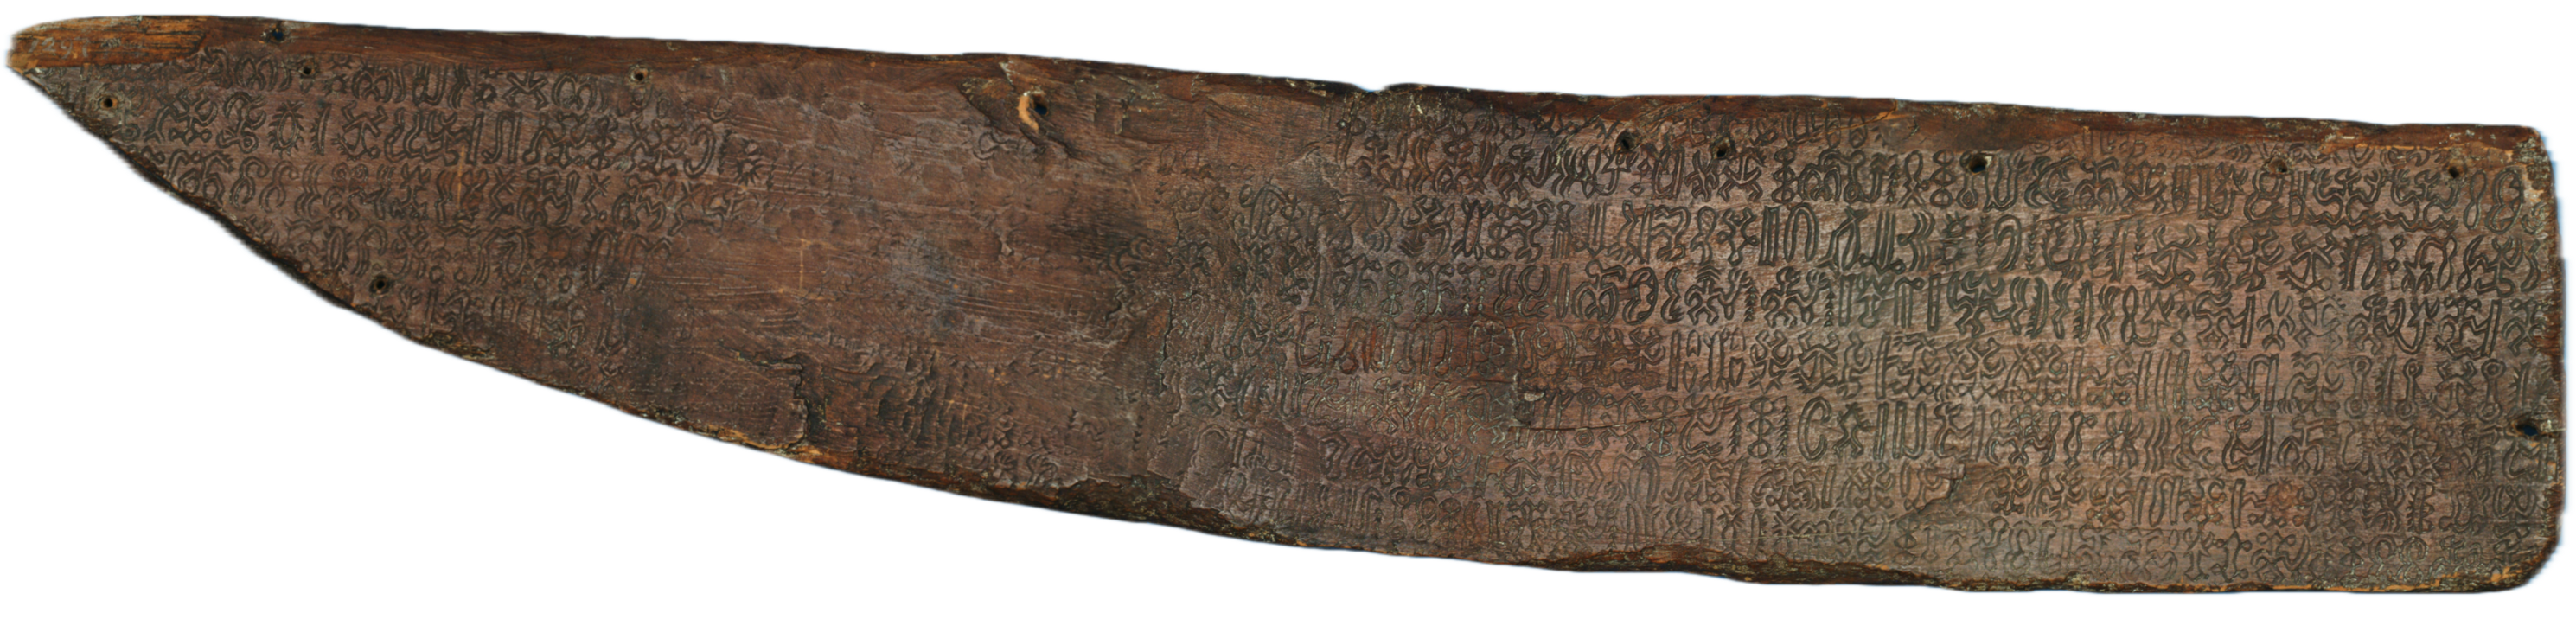
\includegraphics[width=0.9\textwidth]{fig_rongo_g_washington.png}
\caption{\textbf{Rongo Rongo Great Washington Tablet.} Images created by the Smithsonian and compliled by .}
\label{fig_rongo_g_washington}
\end{figure}

\begin{figure}[H]
\centering
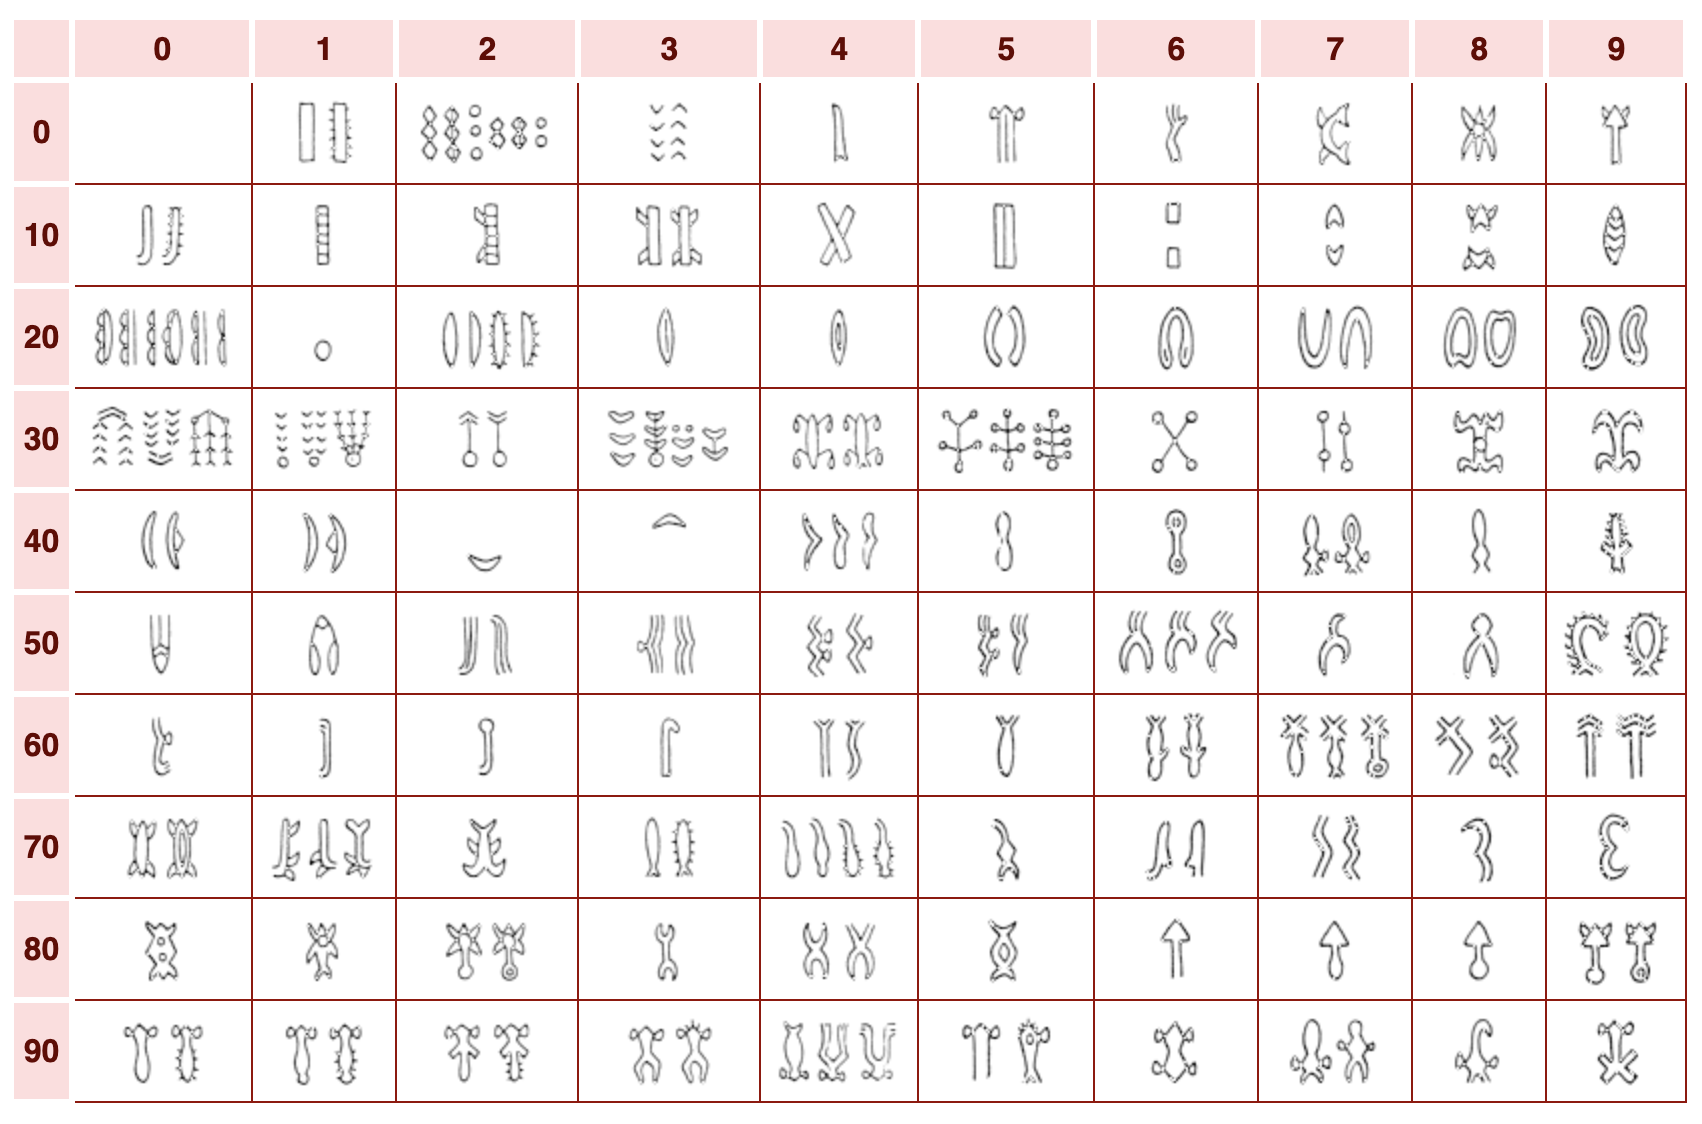
\includegraphics[width=0.9\textwidth]{fig_glyphs_example.png}
\caption{\textbf{Rongo Rongo Glyph Examples.} TODO.}
\label{fig_glyphs_example}
\end{figure}

\subsection{Linear A}


%%%%%%%%%%%%%%%%%%%%%%%%%%%%%%%%%%%%%%%%%%%%%%%%%%%%%%%%%%%%%%%%%%%%%%%%%%%%%%%%%%%
% Methodology and rationale 
%%%%%%%%%%%%%%%%%%%%%%%%%%%%%%%%%%%%%%%%%%%%%%%%%%%%%%%%%%%%%%%%%%%%%%%%%%%%%%%%%%%
\section{Methodology and rationale}
\label{meth}
We apply a machine learning clustering pipeline centered around an HDBSCAN model and information-theoretic techniques as complementary methods. HDBSCAN attempts to group data points into separable clusters by evaluating multivariate similarity among informational features. HDBSCAN is especially useful in unknown languages since it creates separation without requiring labels or a predetermined number of clusters. Information-theoretic measures summarize corpus properties such as uncertainty, redundancy, and properties relevant to decipherability. Shannon entropy measure the uncertainty in the distribution while redundancy 

and entropy-based measures attempt to measure how predictable and redundant each corpus is.  

%%%%%%%%%%%%%%%%%%%%%%%%%%%%%%%%%%
frame the paper as a comparative analysis between ML specific methods (HDBSCAN) and information theoretic (and statistical) methods and compare.

It doesn't matter if these languages are logographic or syllabic, or alien. What I want you to focus on is on what kind of information we can extract from data that we don't know too much about (is agnostic). Assume these are dolphin languages or alien languages.
%%%%%%%%%%%%%%%%%%%%%%%%%%%%%%%%%%%%
\begin{figure}[H]
\centering

\includegraphics[width=0.9\textwidth]{fig_placeholder.png}
\caption{\textbf{TODO.} TODO.}
\label{fig_DS_Process}
\end{figure}

\subsection{Machine Learning}
HDBSCAN
\subsection{Information Theoretical}
Entropy
Unicity Distance
\subsection{Statistical}
TODO

%%%%%%%%%%%%%%%%%%%%%%%%%%%%%%%%%%%%%%%%%%%%%%%%%%%%%%%%%%%%%%%%%%%%%%%%%%%%%%%%%%%
% results
%%%%%%%%%%%%%%%%%%%%%%%%%%%%%%%%%%%%%%%%%%%%%%%%%%%%%%%%%%%%%%%%%%%%%%%%%%%%%%%%%%%
\section{Analysis and Results} 
\label{anal_results}
TODO
%%%%%%%%%%%%%%%%%%%%%%%%%%%%%%%%%%%%%%%%%%%%%%%%%%%%%%%%%%%%%%%%%%%%%%%%%%%%%%%%%%%
% Discussion
%%%%%%%%%%%%%%%%%%%%%%%%%%%%%%%%%%%%%%%%%%%%%%%%%%%%%%%%%%%%%%%%%%%%%%%%%%%%%%%%%%%
\section{Discussion and Future Work}
\label{discussion}

TODO

%%%%%%%%%%%%%%%%%%%%%%%%%%%%%%%%%%%%%%%%%%%%%%%%%%%%%%%%%%%%%%%%%%%%%%%%%%%%%%%%%%%
% appendix
%%%%%%%%%%%%%%%%%%%%%%%%%%%%%%%%%%%%%%%%%%%%%%%%%%%%%%%%%%%%%%%%%%%%%%%%%%%%%%%%%%%
\newpage 
\appendix
\section{TODO}
\label{TODO}

\begin{table}[H]
\centering
\begin{tabular}{p{1.2cm} p{7.5cm} p{3.5cm}}
 \hline
 \rowcolor[gray]{0.95}
 \textbf{Year} & \textbf{Title} & \textbf{TODO} \\ \hline
 2001 & Astronomy and Astrophysics for the New Millennium & Astrophysics \\
 \rowcolor[gray]{0.97}
 2003 & The Sun to the Earth—and Beyond: A Decadal Research Strategy in Solar and Space Physics & Heliophysics \\
 2003 & New Frontiers in the Solar System: An Integrated Exploration Strategy & Planetary  Science \\
 \rowcolor[gray]{0.97}
 2007 & Earth Science and Applications from Space: National Imperatives for the Next Decade and Beyond & Earth Science \\
\end{tabular}
\caption{Decadal Surveys Used in Analysis }\label{tab:Decadals_used}
\end{table}

\section{TODO2}
\label{TODO2}
This section details TODO

\begin{description}
 \item[TODO1:] Follow a \texttt{yyyy-DS-Category-\#\#\#\#.pdf} format where \texttt{\#\#\#\#} is the National Academies document number. \texttt{DS} is used to categorize all Decadal Surveys. \texttt{MA} replaces \texttt{DS} for Midterm Assessments, and \texttt{SP} is used for the Special Publication in 2015 that identified lessons learned.
 
 \item[TODO2:] Follow a \texttt{yyyy\_SSP\_Nasa\_File\_Name.pdf} format. \texttt{SSP} represents Science mission directorate Science Plans. This is replaced with \texttt{AD} to indicate Additional Documentation, \texttt{NSP} to indicate NASA Science Plan, or \texttt{AD} to indicate additional documentation present on the SMD website.
\end{description} 


%% Bibliography
\bibliographystyle{elsarticle-num} 
\bibliography{master.bib}

\end{document}
